%%% -*- coding: utf-8 -*-
\newpage

\chapter{Results}
\label{chap:results}

Having performed 20-fold cross validation, we collected all metrics through all the folds. Table \ref{tab:cross-validation-results} presents mean, standard deviation, min and max. The full results for each fold are available on Table \ref{tab:full-folds}, Appendix \ref{chap:appendix}.

\begin{table}[!ht]
\centering
\caption{Weighted F2-Score (in percentage) for each model across 20-Fold Cross Validation).}
\begin{tabular}{l|l|l|l|l}
      & \multicolumn{1}{c|}{MLP} & \multicolumn{1}{c|}{LSTM} & \multicolumn{1}{c|}{SVM} & \multicolumn{1}{c}{KNN} \\ \hline
count & 20,0000                  & 20,0000                   & 20,0000                  & 20,0000                 \\ \hline
mean  & \textbf{99,0743}                  & 98,9899                   & 98,8993                  & 96,4738                 \\ \hline
std   & 0,1349                   & 0,1174                    & 0,1347                   & 0,2915                  \\ \hline
min   & 98,7945                  & 98,7943                   & 98,5445                  & 95,6932                 \\ \hline
25\%  & 99,0073                  & 98,9175                   & 98,8499                  & 96,3585                 \\ \hline
50\%  & 99,0962                  & 98,9848                   & 98,9174                  & 96,4108                 \\ \hline
75\%  & 99,1708                  & 99,0684                   & 98,9756                  & 96,6564                 \\ \hline
max   & 99,2885                  & 99,1915                   & 99,0836                  & 96,9448                
\end{tabular}
\label{tab:cross-validation-results}
\end{table}

\section{Model comparisson}\label{sec:comparisson}
Comparing the models in Table \ref{tab:cross-validation-results} the model with the highest mean weighed F2-Score across folds is the Multilayer Perceptron model. To compare the models and test if their results are statistically different. 

Afterwards, we test if the model with the best model has a statistically significant difference from the second best by performing a post-hoc pairwise hypotesis test.

\begin{figure*}[!ht]
    \centering
    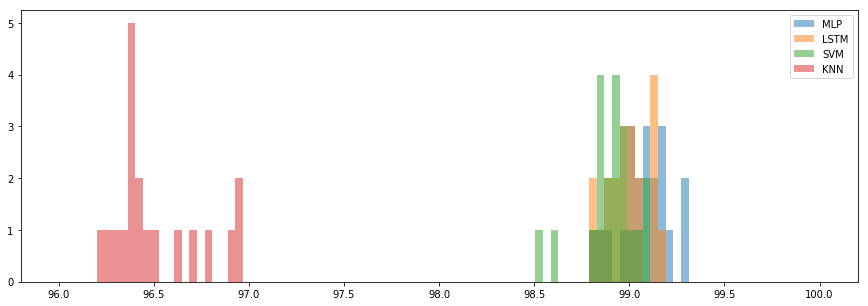
\includegraphics[width=0.9\textwidth]{img/results/histogram.png}
    \caption{Histogram of the results of each model throughout the 20-fold cross validation.}
    \label{fig:results-histogram}
\end{figure*}

Figure \ref{fig:results-histogram} shows the difference in the distribution of results of each model. The simplest model, K-Nearest Neighbors, has the most difference from the models. The three other models, however, are relatively close to each other.

To determine what test is better suited for our data distribution (the best weighed F2-Score), we checked our data for normality and outliers. Which are frequent assumptions for different hypothesis tests.
For the normality assumption we used probability plots, as shown in Figure \ref{fig:prob-plots} to test if the data is normal.

\begin{figure*}[!ht]
    \centering
    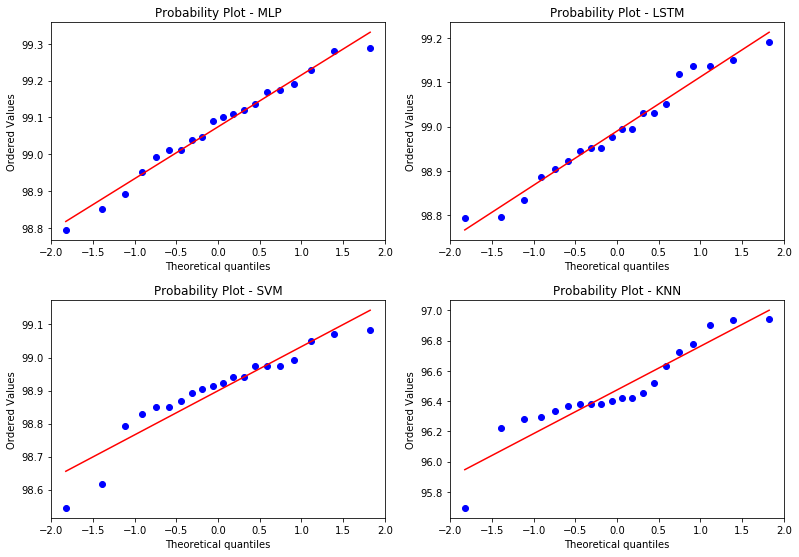
\includegraphics[width=0.8\textwidth]{img/results/pp-plot.png}
    \caption{Probability plots for each model, it shows the data's quantiles against the quantiles of a theoretical distribution (the normal distribution).}
    \label{fig:prob-plots}
\end{figure*}

As shown in Figure \ref{fig:prob-plots}, the KNN and SVM models differ from a normal distribution. 

In order to validate what is shown in the probability plots, we also tested the normality assumption with the Shapiro-Wilk test. The null hypotesis is that the data is not drawn from a normal distribution. The alternative hypotesis is that the data is drawn from a normal distribution.

According to the Shapiro-Wilk test, the MLP and LSTM models follow a normal distribution (p<0.05). As for the SVM and KNN models, they do not follow a normal distribution (p>0.05). So our data does not support tests that requires data with normal distribution.

\begin{figure*}[!ht]
    \centering
    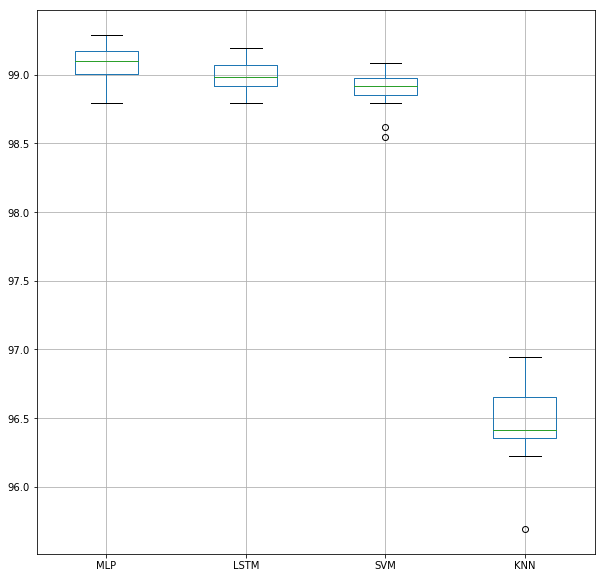
\includegraphics[width=0.5\textwidth]{img/results/boxplot.png}
    \caption{Boxplot of the results of each model throughout the 20-fold cross validation.}
    \label{fig:results-boxplot}
\end{figure*}

For outliers presence, as seen by the box plot in Figure \ref{fig:results-boxplot}, there are outliers in the SVM and KNN data.

When tested with of most parametric tests, both outliers and non-normal distributions can bias the results and potentially lead to incorrect conclusions if not handled properly.

To choose a test, we chose a non-parametric (sample median) test, because sample medians are less sensitive to outliers, in contrast with the mean or variance based parametric tests, such as Variance Analysis (ANOVA).
%https://www.reneshbedre.com/blog/kruskal-wallis-test.html
We defined the null hypothesis as "All models folds evaluations medians are equal"; The alternative hypothesis is that "At least one model mean rank (median) is different from other groups".
We used a two-tailed test since we do not know which model will be higher.
Our chose our alpha as 0.05. That is, a probability of 5\% of committing a error, rejecting the null hypothesis when it should be accepted.

We chose the Kruskal-Wallis test \cite{kruskal1952use} as our hypothesis test because it fits all of our requisites (non-parametric, median based). Our data also supports all of this test's assumptions.

After applying the Kruskal-Wallis test we obtained a p-value of 2.2733e-11, which means that p<0.05 and that we can reject the null hypothesis and accept the alternative hypothesis.

To determine which models are statistically different from each other, we performed a post-hoc test using the Nemenyi post hoc test \cite{nemenyi1963distribution}, because it is a non-parametric (distribution free) test and our data does not follow a normal distribution. The results from this test are presented in Figure \ref{fig:significance-matrix}.

\begin{figure*}[!ht]
    \centering
    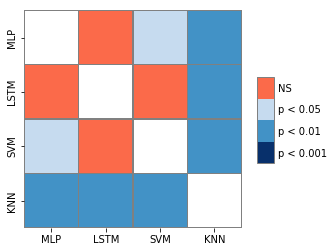
\includegraphics[width=0.5\textwidth]{img/results/significance-matrix.png}
    \caption{Significance matrix. Plot made with scikit-posthocs\cite{Terpilowski2019}.}
    \label{fig:significance-matrix}
\end{figure*}

As presented in Figure \ref{fig:significance-matrix}, the MLP and LSTM models are not significantly different from each other (p>0.05) and that the KNN model is statistically different from all other models (p<0.05).

\section{Tests results}\label{sec:tests}

We tested the best performing model, the Multilayer-Perceptron, on the test subset, shown in Table \ref{tab:test-general-results}. 

\begin{table}[!ht]
\centering
\caption{Test subset results, shown in absolute values).}
\begin{tabular}{l|l|l|l|l|l}
             & precision & recall & f1-score & f2-score & support                         \\ \hline
Safe         & 0,9895    & 0,9906 & 0,9900   & 0,9897   & 5973,0000                       \\ \hline
Sensitive    & 0,9906    & 0,9895 & 0,9900   & 0,9904   & 5973,0000                       \\ \hline
weighted avg & 0,9900    & 0,9900 & 0,9900   & 0,9900   & \multicolumn{1}{l}{11946,0000}
\end{tabular}
\label{tab:test-general-results}
\end{table}

As shown in Table \ref{tab:test-general-results} and in Figure \ref{fig:cf-test}, the MLP model has performed within the range of the mean of the cross validation. It can also be noted that, the most frequent errors were \textit{false positives}, when the model predicted a video as Sensitive when it was in fact, Safe. 

\begin{figure*}[!ht]
    \centering
    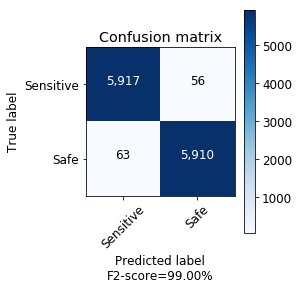
\includegraphics[width=0.49\textwidth]{img/results/MLP-TEST.png}
    \caption{Confusion matrix of the predictions of the best model in the test subset.}
    \label{fig:cf-test}
\end{figure*}

We also tested our best model in each sub task, pornography and gore binary classification. For the pornography, shown in Table \ref{tab:test-porn-results}, and Figure \ref{fig:cf-test-porn}, the most frequent error were the \textit{false negatives}, in which the model predicted that the most samples were predicted as Safe, but were actually Sensitive. 

\begin{table}[!ht]
\centering
\caption{Results testing pornography only, shown in absolute values).}
\begin{tabular}{l|l|l|l|l|l}
             & precision & recall & f1-score & f2-score & support    \\ \hline
Safe         & 0,9947    & 0,9902 & 0,9925   & 0,9939   & 5737,0000  \\ \hline
Sensitive    & 0,9903    & 0,9948 & 0,9925   & 0,9911   & 5737,0000  \\ \hline
weighted avg & 0,9925    & 0,9925 & 0,9925   & 0,9925   & 11474,0000
\end{tabular}
\label{tab:test-porn-results}
\end{table}

For the gore, shown in Table \ref{tab:test-gore-results}, and Figure \ref{fig:cf-test-gore}, the most frequent error were the \textit{false positive}, in which the model predicted that the most samples were predicted as Sensitive, but were actually Safe.  

\begin{table}[!ht]
\centering
\caption{Results testing gore videos only, shown in absolute values).}
\begin{tabular}{l|l|l|l|l|l}
             & precision & recall & f1-score & f2-score & support  \\ \hline
Safe         & 0,8764    & 0,9915 & 0,9304   & 0,8834   & 236,0000 \\ \hline
Sensitive    & 0,9902    & 0,8602 & 0,9206   & 0,9661   & 236,0000 \\ \hline
weighted avg & 0,9333    & 0,9258 & 0,9255   & 0,9248   & 472,0000
\end{tabular}
\label{tab:test-gore-results}
\end{table}

\begin{figure*}[!ht]
    \centering
    \begin{subfigure}[b]{0.49\textwidth}
        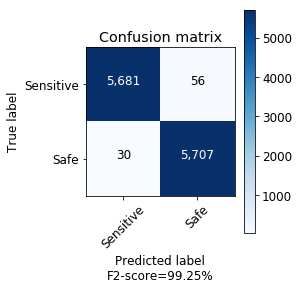
\includegraphics[width=0.93\textwidth]{img/results/MLP-TEST-PORN.png}
        \caption{Confusion matrix of the model on the pornography videos of the test subset.}
        \label{fig:cf-test-porn}
    \end{subfigure}
    \begin{subfigure}[b]{0.49\textwidth}
        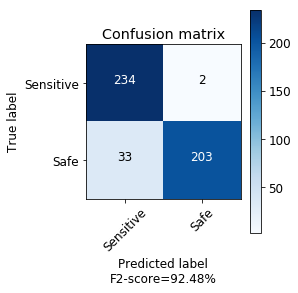
\includegraphics[width=0.90\textwidth]{img/results/MLP-TEST-GORE.png}
        \caption{Confusion matrix of the model on the gore videos of the test subset.}
        \label{fig:cf-test-gore}
    \end{subfigure}
    \caption{Confusion matrices of the best performing model on the pornography and gore subsets.}
\end{figure*}

To evaluate if our model and our dataset on the pornography detection (binary classification) task, we also tested our best performing baseline model on a well known dataset for pornography detection: The 2k-pornography dataset. The results are shown in \ref{tab:test-2k-results} and in Figure \ref{fig:cf-test-2k}. The most common errors were false negatives, in which the model predicts the instance as a Safe, but the true label were Sensitive.

\begin{table}[!ht]
\centering
\caption{Test on the NPDI 2k-pornography dataset results, shown in absolute values).}
\begin{tabular}{l|l|l|l|l|l}
             & precision & recall & f1-score & f2-score & support    \\ \hline
Safe         & 0,9665    & 0,8080 & 0,8802   & 0,9411   & 1.000,0000 \\ \hline
Sensitive    & 0,8351    & 0,9720 & 0,8983   & 0,8354   & 1.000,0000 \\ \hline
weighted avg & 0,9008    & 0,8900 & 0,8893   & 0,8883   & 2.000,0000
\end{tabular}
\label{tab:test-2k-results}
\end{table}

\begin{figure*}[!ht]
    \centering
    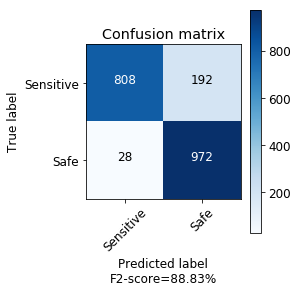
\includegraphics[width=0.49\textwidth]{img/results/MLP-2K-TEST.png}
    \caption{Confusion matrix of the predictions of the best model in the NPDI 2k-pornography dataset.}
    \label{fig:cf-test-2k}
\end{figure*}

\section{Analysis cases}\label{sec:experiments-discussion}

As detailed in analysis \textbf{(E0)} and \textbf{(E1)} (Section \ref{sec:experiments}), in order to further investigate the impact of each multi-modal feature in our best performing model, the Multilayer Perceptron. We tested it on our test subset and on the NPDI 2k-pornography dataset, but only using one modal feature at a time. For example, in Figure \ref{fig:cf-test-image}, we tested the MLP model using only visual (frames) features, specifically, were changed all audio features for zero to simulate a video with no audio features.

\begin{figure*}[!ht]
    \centering
    \begin{subfigure}[b]{0.49\textwidth}
        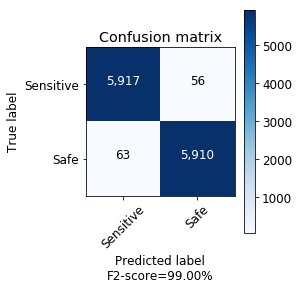
\includegraphics[width=0.94\textwidth]{img/results/MLP-TEST-IMAGE-ONLY.png}
        \caption{Confusion matrix of the model on the test subset using only image features.}
        \label{fig:cf-test-image}
    \end{subfigure}
    \begin{subfigure}[b]{0.49\textwidth}
        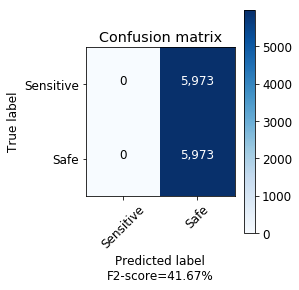
\includegraphics[width=0.94\textwidth]{img/results/MLP-TEST-AUDIO-ONLY.png}
        \caption{Confusion matrix of the model on the test subset using only audio features.}
        \label{fig:cf-test-audio}
    \end{subfigure}
    \caption{Confusion matrices of the model on the test subset using only one multi-modal feature at a time.}
\end{figure*}

As observed in Figures \ref{fig:cf-test-image} and \ref{fig:cf-test-audio}, our model had the same performance with only visual features, but mis-classified all Sensitive videos. This means that the MLP model ignored all audio features for all videos. It is relying only in visual features, even though there are examples of videos in the dataset, in which the main feature of a sensitive video is audio. % ASMr VIDEOS

\begin{figure*}[!ht]
    \centering
    \begin{subfigure}[b]{0.49\textwidth}
        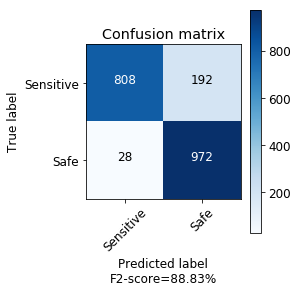
\includegraphics[width=0.94\textwidth]{img/results/MLP-2K-TEST-IMAGE-ONLY.png}
        \caption{Confusion matrix of the model on the NPDI 2k-pornography dataset using only image features.}
        \label{fig:cf-test-2k-image}
    \end{subfigure}
    \begin{subfigure}[b]{0.49\textwidth}
        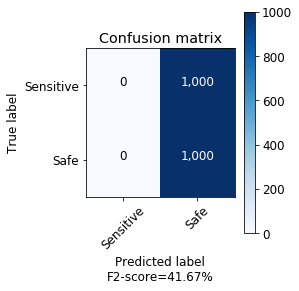
\includegraphics[width=0.94\textwidth]{img/results/MLP-2K-TEST-AUDIO-ONLY.png}
        \caption{Confusion matrix of the model on the NPDI 2k-pornography dataset using only audio features.}
        \label{fig:cf-test-2k-audio}
    \end{subfigure}
    \caption{Confusion matrices of the model on the NPDI 2k-pornography dataset using only one multi-modal feature at a time.}
\end{figure*}

As described in analysis \textbf{(E2)} and \textbf{(E3)} (Section \ref{sec:experiments}), we confirmed the same pattern in the tests with the NPDI 2k-pornography dataset, as shown in Figures \ref{fig:cf-test-2k-image} and \ref{fig:cf-test-2k-audio}.%, our model relied only in visual features.

% Discutir vantagens e desvantagens do eraly fusion por causa de forçar o modelo a aprender uma mdeia de cada e depois combinar
% Possibilidades pra so ter aprendido imagens:
%Diferença no tamanho das deatures de audio e frames
%Diferença pra early e late fusion
%Só a mlp aprendeu isso
%Features ruins de audio
% Receptive field pra áudio pequeno
% Audio n faz diferença ***: perguntar pra paulo oq ele quis dizer
Because of the late fusion approach, in which the model receives both feature types and decides which ones to use the most we were susceptible to this learning behavior.
There are multiple reasons that could explain these results:
\begin{itemize}
    \item The difference in the size of visual features and audio features (1024 for visual and 128 for audio);
    \item This specific model learned to ignore the audio features;
    \item The audio features did not offer as much differentiation power as much as the visual features in this dataset.
    \item The audio feature extraction method did not offer as much differentiation power as the visual features.
\end{itemize}

To use late fusion in the multimodal features could improve our performance in this task because a model is trained for each multimodal feature, assuring use of each available feature type.

\section{Discussion}\label{sec:discussion}
% Falar dos resultados de teste e de cada task
When testing the best performing model, the MLP, there was little variation on the test subset performance. One explanation to this could be that our dataset is mostly homogeneous (Does not have much variation in videos characteristics). This could also be a consequence of the dataset's sampling, resulting in a test subset similar to the train/validation subset.  However, there steps taken to avoid both these possibilities. The dataset was created with a wide variety of videos within each subclass, such as education and sports for the safe videos, and the test subset was a random sampling that followed the distribution of main tags within each of subclasses.
% Para tarefas de porn, o mais comum foram falsos negativos, como esperado
On the pornography detection task, the results were still within the expected performance and the most frequent errors were false negatives, which is an error we want no minimize the most over false positives.
% Para tarefas  de gore, o mais comum foram falsos positivos, que previram como sensivel mas eram safe, que é o idela, mas pq esses videos sao bem parecidos com safe
On the gore detection task, there was a significant performance drop, which could be a reflection of the smaller amount of gore examples in the dataset, or could mean that this approach is less adequate to the gore detection task than to the pornography detection task.

% Falar dos erros do pornography2k, que usou f2 score, de quanto foi o modelo deles, e dos erros mais comuns (Falsos negativos) 
When testing the best performing model on the NPDI 2k-pornography dataset, there was a significant drop in performance compared the test subset, this could possibly be due to the model's lack of use of audio features. This could also mean that our dataset misses specific hard instances of either class.

% Falar pq isso aconteceu, qual a diferença entre os dois datasets e os modelos
% por eles usarem late fusion talvez tenha ajudado, especialmente pq o nosso modelo usa só as features de imagem

